
\documentclass[11pt,a4j,titlepage,oneside]{jsbook}


\usepackage[dvips]{graphicx}
\usepackage{fancyhdr}
\usepackage{amsmath,amsthm,amssymb}
\usepackage{base}
\usepackage{times,mathptmx}
\usepackage{dcolumn,multirow,ccaption}


\newcolumntype{.}{D{.}{.}{-1}}



\usepackage{tabularx}
\usepackage{ascmac}

    % ref.http://www.spa.sys.eng.shizuoka.ac.jp/~tanaka/tex/tech/screen.html

\setcounter{tocdepth}{2}
\setlength{\textwidth}{45zw}

\renewcommand{\arraystretch}{0.8}



\year{平成28年度 学士論文}
\title{ハンガリアン法による語の相似関係抽出}
\titleE{Analogous word association and its detection by the Hungarian method.}
\author{平田 泰樹}
\date{2017年2月10日}
\authorE{Taiki Hirata}
\lab{北海道大学 工学部 情報エレクトロニクス学科 コンピュータサイエンスコース 知識ベース研究室}
\labE{Department of Electronics and Information Engineering. \\Hokkaido University}



\begin{document}


\maketitle

\pagestyle{plain}
\cleardoublepage
\pagenumbering{roman}




\tableofcontents
\listoffigures
\listoftables

\cleardoublepage
\pagenumbering{arabic}
\pagestyle{headings}


\chapter{序論}

\section{はじめに}
SNSなどのサービスが普及し、以前にも増して世界中の人々がインターネット上にテキストデータを投稿するようになった。こうして集められるデータは、その人の趣向、動向、人と為りや、世界の動向を知る手掛かりとなるだろう。しかし、インターネット上にあるテキストデータは膨大なものになっており、ユーザーが本当に欲しい情報は見えにくく、扱いづらいものとなってしまっている。\\
膨大なデータを有効活用していくためには、効率的な分類、加工をしていかなければならないが、データのすべてを人手で解析し、まとめることは非常に困難である。そこで、計算機を利用してこのテキストデータを処理することがさまざまな分野で考えられている。
\\
テキストデータを計算機で処理するにあたって、テキストを何らかの方法で数値化する必要がある。そもそもテキストを構成する文字自体は単なる記号であり、また、計算機が文字データを識別するために、文字一つ一つに事前に割り当てられている数値には、記号識別以上の意味がない。\\
そこで、テキストを計算機で処理するために、いかにして意味を持つ数値で表現し、どのように利用するか、が課題となっている。
\\
\section{研究背景}
テキストを、意味を持つ数値で表現する手法について、現在まででいくつかの方法が研究されている。中でも2013年に発表されたword2vecは、ニューラルネットワークによって学習した単語の意味表現ベクトルで、単語の和、差の計算ができるようになり話題となった。\\
\\
このベクトルの加算減算が可能になったこと、形態素ベクトルの位置関係に相似性が見られることは、主成分分析、t-SNEなどで次元を削減し、可視化したデータから見て取れる。
\\
\section{本研究の目的}
本研究では、word2vecにより得たベクトルデータを可視化することなしに、語の相似関係を抽出することを目的としている。
\\
\section{本論文の構成}
はじめに本章は序論であり、研究背景に関して述べた。\\
本稿2章では、本研究で用いる単語の意味表現についての説明を述べた。
3章では、本研究で用いるベクトルデータを出力するword2vecについて述べた。\\
4章では、word2vecにより得られたデータの解析に用いる、梅山氏のグラフノードマッチング問題に関する提案手法と、ハンガリアン法について述べた。\\
5章で、本研究で行った実験の流れについて説明し、結果を検証した。\\
最後に6章では、本研究における結論と、今後の展望について考慮していることを述べて最後のまとめとした。\\


\chapter{意味表現の学習}
本研究では、word2vecで学習した分散表現ベクトルから語の相似関係を抽出することを目的としている。本章では、単語の意味表現の学習についていくつかの表現方法と、word2vecで可能な分散表現ベクトルについてを説明する。

\section{形態素と意味表現}
\subsection{形態素}
自然言語とは、人と人とのコミュニケーションに用いられる道具であり、文字、あるいは音の並びによって構成されている。しかし、一般に文字、或いは音そのものは意味を持たないため、自然言語の最小単位として\textbf{形態素}を用いることが多い。\\
形態素とは、文字列が意味、或いは役割を持つ最小のまとまりである。本研究ではこの形態素に着目していく。

\subsection{形態素解析}
多くの自然言語処理に関わるタスクは、形態素を最小単位としているが、日本語などの言語は特に、形態素ごとに区切られた文章ではなく、また、計算機は、形態素のまとまりを認識できない。そこで、自然言語処理をする際に、第一の処理として\textbf{形態素解析}を行うのが一般的である。\\
形態素解析の目的は、入力された文を、形態素毎に区切り、品詞などを決定することである。

本研究では、京都大学情報学研究科と、日本電信電話株式会社コミュニケーション科学基礎研究所が、共同研究ユニットプロジェクトで開発した\textbf{MeCab}\footnote{http://taku910.github.io/mecab/}\cite{mecab}という、オープンソースの形態素解析エンジンを実験データの前処理に用いた。

\subsection{意味表現}
自然言語を計算機で処理するにあたって、計算機が形態素の意味や役割を獲得すれば、文や文章など、より複雑な構造の意味を理解し、それに応じた処理ができるようになることが期待されている。この、計算機で認識するために形態素の意味や役割を何らかの数値で表現したもの、或いは表現することを意味表現という。\\
では、意味表現をどのように与えるかということが問題になる。

\section{辞書}
我々は、未知語の意味を知ろうとする時に検索エンジンでの意味を調べるなど、何らかの方法で意味が記述されたものを参照する。その参照対象をここでは一括して辞書と呼ぶこととする。辞書を計算機に与えることで、意味を教えることはできるかもしれない。日本語\textbf{WordNet}\footnote{http://nlpwww.nict.go.jp/wn-ja/}は、計算機で使うことを想定して開発された辞書である。

\subsection{WordNet}
日本語版WordNetは国立研究開発法人情報通信研究機構(NICT)で2006年から2012年まで開発されていた大規模な日本語意味辞書である。プリンストン大学で開発されたPrinceton WordNetと、ヨーロッパのEuroWordNet協会が推進するGlobal WordNet Gridに着想を得て開発された。\\
WordNetでは、単語の意味を\textbf{synset}と呼ばれるグループで表現しており、各synsetは単語の意味に関する記述と、上位関係や下位関係など、他のsynsetとの関係などが保持されている。なお、今回使用しているこの日本語WordNetの情報規模は以下の通りである。\cite{j_WordNet}
\begin{itemize}
  \item{synset数} 57,238
  \item{単語数} 93,834
  \item{語義数:synsetと単語のペア} 158,058
  \item{定義文数} 135,692
  \item{例文数} 48,276
\end{itemize}

人手で整備された辞書は単語の意味に関してある程度精密な情報を備えているが、新語や、多くの複合語には対応しきれておらず、たとえば、MeCabを用いて日本語版Wikipedia全文から抽出された形態素数は63〜84万程度であった。(数字の幅があることに関しては後ほど説明するが、形態素の基本形で数えた場合と、活用された形そのままの場合の2パターンで実験をしたからである。)こうした点から、単語・複合語のすべてとすべての意味を収録し、あらゆる言語処理の応用に耐えうる辞書を作成することは、非常に困難であることがわかる。

\newpage

\section{統計的手法}
辞書などを作成することで、計算機に単語の意味を明示的に与えることには限界があることがわかった。そこで、現在数多くある、人間が生み出したテキストデータから自動的に単語の意味を学習・獲得させることを考える。

\subsection{分布的意味表現}
まず一つに\textbf{分布的意味表現}というものがある。\\
これは、\textbf{分布仮説}
\begin{quote}
  The Distributional Hypothesis is that words that occur in the same contexts tend to have similar meanings(Harris, 1954). (ACL wiki)
\end{quote}
”同じ文脈に出現する単語は、似た意味を持つ。”
という考え方によって構築されるものである。\cite{JRFirth}

\begin{figure}[h]
  \centering
  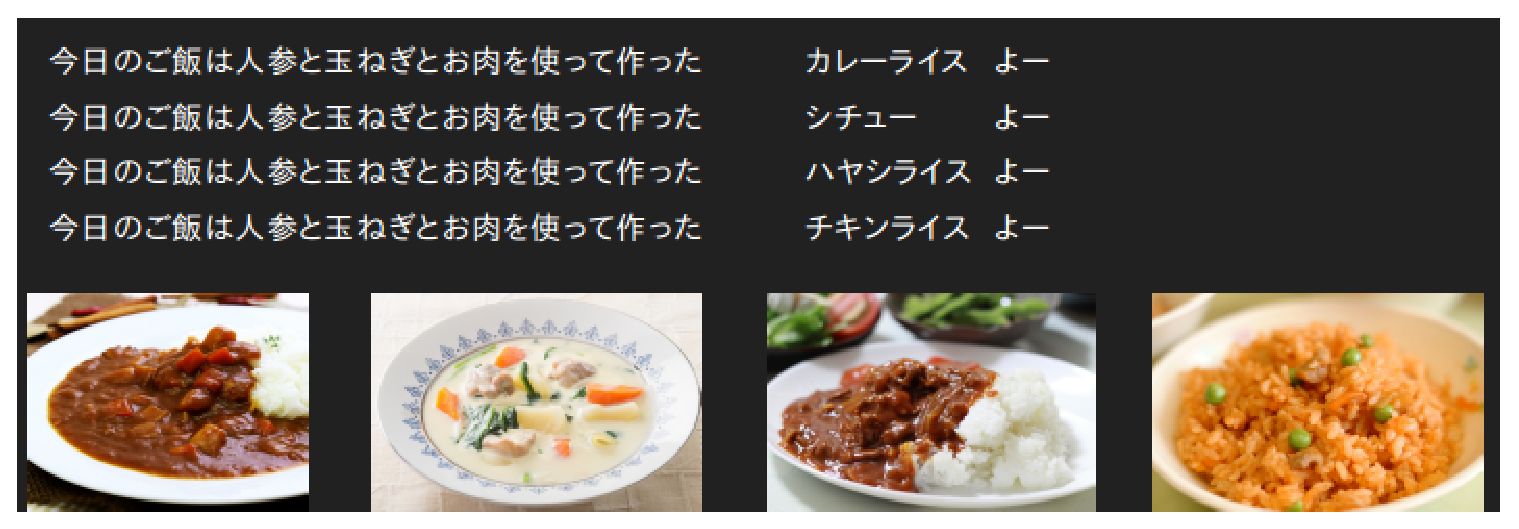
\includegraphics[width=15cm]{../images/kyou_gohan.eps}
  \caption{分布仮設による意味の類推例}
\end{figure}

上述の例は全く同じ文脈で、似たような料理名が出てくる例文を並べたものである。この時、もしどれかひとつの料理名が全く無知なものであったとしても、それが料理であること、どのようなものであるか、ある程度類推することができるだろう。それは、まさしく同じ文脈に出現する単語であるからに違いない。\\
\\
この考えに則ってベクトルを作成してみる。例えば、
\begin{itemize}
  \item 今日の晩御飯は、ジャガイモの入ったカレーライスだ。
  \item 今日の晩御飯はハヤシライスだ。
\end{itemize}
という二本の文章を例にして、”カレーライス”と”ハヤシライス”の意味表現を考える。\\
\\
まず、それぞれの文章を形態素解析すると、

\begin{itemize}
  \item $今日 \backslash の \backslash 晩御飯 \backslash は \backslash 、 \backslash ジャガイモ \backslash の \backslash 入っ \backslash た \backslash カレーライス \backslash だ \backslash 。$
  \item $今日 \backslash の \backslash 晩御飯 \backslash は \backslash ハヤシライス \backslash だ \backslash 。$
\end{itemize}
となる(上では $\backslash$ によって形態素を区切っている)。

これをもとに、”カレーライス”と”ハヤシライス”に関して、同じ文脈に着目した意味表現ベクトルを作成する。\\
\\
同じ文脈に出現する形態素(これ以降文脈語と呼ぶ)をベクトルの各次元とし、注目する単語と何個の同じ文脈でその次元の文脈語が出現しているかを値としてとると、
\begin{itemize}
  \label{weight_equation}
  \item $カレーライス = [(今日:1),(の:1),(晩御飯:1),(は:1),(、:1),(ジャガイモ:1),(入っ:1),(た:1),(だ:1),(。:1)]$
  \item $ハヤシライス = [(今日:1),(の:1),(晩御飯:1),(は:1),(、:0),(ジャガイモ:0),(入っ:0),(た:0),(だ:1),(。:1)]$
\end{itemize}
と表すことができる。\\

ここで、ある単語$x_i$と別な単語$x_j$が何らかの文脈で同時に出現していることを\textbf{共起}していると言い、何度共起しているかの回数を\textbf{共起頻度}と言う。つまり、上記の例で作成したベクトルは、共起頻度を値として持つ\textbf{共起ベクトル}である。\cite{book_wm}この方法でベクトルを作成する場合は、学習に用いられるテキストの集まり\textbf{コーパス}すべてから学習するため、一般に高次元で疎なベクトルが生成される。これは、コーパスに含まれる単語数が数万程度であったり、単語数に対し、語が共起することは多くないためである。

こうして作成される意味表現ベクトルを用いて別な自然言語処理のタスクを行う際、元々のベクトルが高密度で疎なものであるために、学習事例を正しく表現できなくなってしまうなどの問題が発生してしまう。

\subsection{分散的意味表現}
分布的意味表現ベクトルが高次元で疎なものであるという点を避けた学習方法として提案されたのが、\textbf{分散的意味表現}である。\\
\\
分散的意味表現の学習手法の基本は以下のようになっている。\\
\begin{enumerate}
  \item まず、すべての単語に、任意の固定次元のベクトルを割当て、ランダムな実数値で初期化する。
  \item 与えられたベクトルを用いて、何らかの予測タスクを解く。
  \item 予測タスクを解いた結果に応じてベクトルの値を更新する。
  \item 2へ戻る。
\end{enumerate}

分散的意味表現を表すベクトルの各次元は、何らかの実数値変数が持つ値と解釈することができる。この実数値変数が持つ特徴はどのような予測タスクを解くか、固定次元数をどのくらいの値にするかなどによって変わると予想されるが、単純な共起頻度が値となるわけではなく、また、他の様々な形態素と次元を共有することから、コーパス中で共起することがない形態素同士の関係についても表現できることが期待される。

次章では、本研究で用いた形態素の分散的意味表現学習ツールword2vecで実装されている2種類の予測タスクについて述べる。


\chapter{word2vec}
\textbf{word2vec}\footnote{https://github.com/svn2github/word2vec}とは、2013年にGoogleのMikolovらが発表した、単語の分散的意味表現学習ツールである。意味表現学習の過程で解くのは、ある文脈内で共起する形態素を予測するタスクである。文脈が与えられ、次に出てくる形態素を予測するモデルを\textbf{言語モデル}と言い、これは、与えられた形態素列がどれほどその言語らしいかを評価するモデルである。

言語モデルでは着目形態素の前方にある形態素のみから次に来る形態素を予測しなければならないが、意味表現獲得を目的とする場合、後方の形態素も予測に使うことができる。よって、$x_1,...,x_{i-1}$と、$x_{i+1},...,x_n$から$x_i$を予測する。

この章ではword2vecに実装されている2つの手法を紹介していく。

\section{実装アルゴリズム}
それぞれの手法を紹介していく前に事前に確認しておくが、word2vecでは、単語の予測タスクを解く上で、一つの単語に対し、二つのベクトルを設定し、学習を進めている。以下に述べる二つの手法の双方で、同一文脈における単語の共起を、意味表現ベクトルの内積で定義しているためである。

通常同一単語が同一文脈に出現することは稀であり、$x_i$に着目した時、$x_i$の文脈で$x_i$が出現する確率$p(x_i|x_i)$を小さくする必要があるが、この確率を導出する計算過程で$x_i^Tx_i$を計算することになる。そして、$p(x_i|x_i)$を小さくするために、$x_i^Tx_i$を小さくしなければならない。しかし、この後に述べるが$p(x_i|x_i)$の導出にはソフトマックス関数という関数を利用しており、これはスケール不変な関数で、$x_i^Tx_i$を小さくしても値が変化しない。

こうした問題を避けるために、以下の手法中では、用いる意味表現ベクトルを、同じ単語が対象語として現れるか、対象語と共起する文脈語として現れるかによって使い分けている。

\subsection{連続単語袋詰モデル}
\textbf{連続単語袋詰モデル}(Continuous Bag-of-Words model, CBoW model)では、\textbf{文脈語}(着目形態素と共起している形態素)から着目形態素の出現確率を予測している。
\begin{figure}[h]
  \centering
  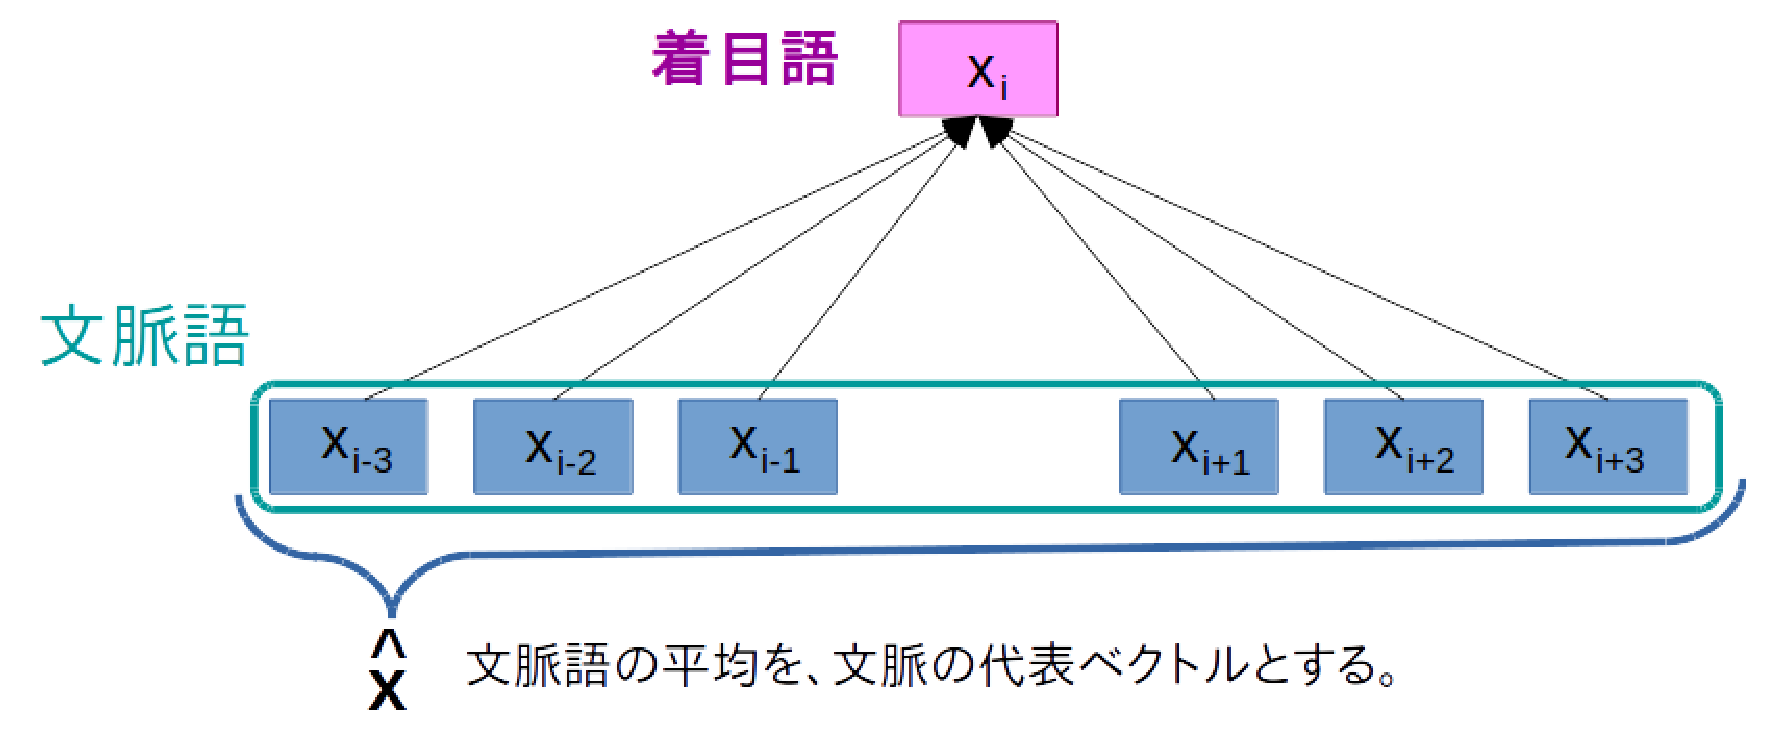
\includegraphics[width=12.5cm]{../images/CBoW.eps}
  \caption{CBoWによるベクトル構築イメージ}
\end{figure}

着目形態素の前後n(下図では3)個の形態素を文脈語とし、文脈語の表現ベクトルの平均を、着目形態素$x_i$の文脈を代表するベクトル$\hat{x}$として、与えられた文脈中に、着目形態素$x_i$が出現する確率$p(x_i|\hat{x})$は、
\begin{eqnarray}
  \label{cbow_p}
  p(x_i|\widehat{x}) = \frac{\exp(\hat{x}^Tx)}{\sum_{x'\in\nu}\exp(\hat{x}^Tx')}
\end{eqnarray}
と表せる。ここで$\nu$はコーパス中の全形態素からなる語彙集合であり、x'は$\nu$中の単語である。\\
文脈語の代表ベクトル算出時に語順を無視しているため、同じく語順を無視して文や文書ベクトルを導出する\textbf{Bag-of-Wordsモデル}の拡張とみなすことができる。

式(\ref{cbow_p})で導出できる確率を学習していく。学習過程については、次のモデルで学習する確率を説明した後に述べる。

\subsection{連続スキップグラムモデル}
\textbf{連続スキップグラムモデル}(continuous Skip-gram model, Sg model)では、連続単語袋詰モデルとは逆に、与えられた文脈語から着目形態素の出現を予測するものとなっている。
\begin{figure}[h]
  \centering
  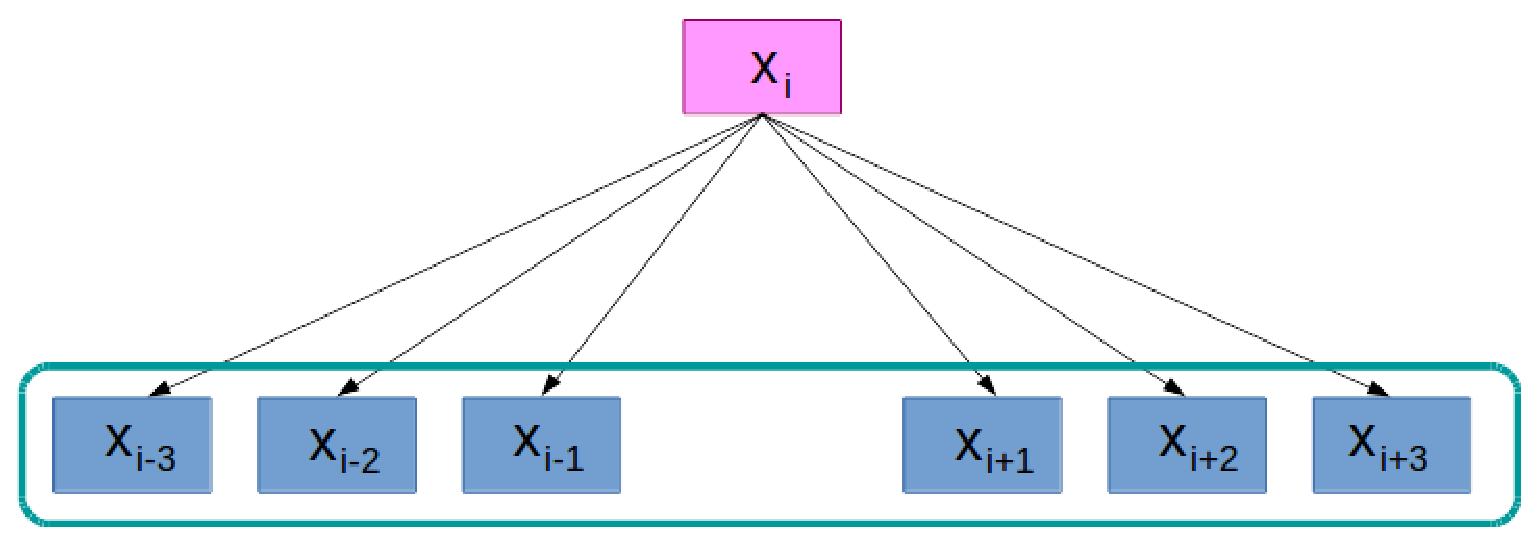
\includegraphics[width=12.5cm]{../images/Sg.eps}
  \caption{Sgによるベクトル構築イメージ}
\end{figure}

着目形態素$x_i$から文脈語を予測する場合の確率$p(z_{i-n},...,z_{i-1},_{i+1},...,z_{i+n}|x_i)$は、着目形態素$x_i$が与えられた時、文脈語$z_{i-n},...,z_{i-1},z_{i+1},...,z_{i+n}$の出現確立がすべて独立であると仮定して、
\begin{eqnarray}
  \label{cskip_p}
  p(z|x_i) = \frac{\exp(x_i^Tz)}{\sum_{z'\in\nu(x)}\exp(x^Tz')}
\end{eqnarray}
と表せる。ここで$\nu(x)$はコーパス中で着目形態素$x_i$と共起している文脈語の集合であり、zは文脈語ベクトルである。\\
文脈語の独立性を仮定することで、
\begin{eqnarray}
  p(z_{i-n},...,z_{i-1},z_{i+1},...,z_{i+n}|x_i) = p(z_{i-n}|x_i)...p(z_{i-1}|x_i)p(z_{i+1}|x_i)...p(z_{i+n}|x_i) \nonumber
\end{eqnarray}
と表すことができ、スキップグラムモデルでの確率計算を簡単にしている。

\subsection{二つの学習モデルの違い}
連続スキップグラムモデルでは、一つの着目形態素と一つの文脈語の関係から確率計算を行うので、少ないコーパスからでも一定の精度のモデルを学習できる。これに対し連続単語袋詰めモデルでは複数の文脈語から一つの着目形態素を予測するモデルであるため、複数の文脈語からなる単語列が、コーパス中に複数回出現している必要がある。したがって、連続スキップグラムモデルよりも大きなコーパスデータが必要となる。\cite{book_wm}

\section{モデルの最適化}
本節ではいよいよ、前節で導出した確率の最適化について述べていく。

まず、式(\ref{cbow_p}),(\ref{cskip_p})の右辺は\textbf{ソフトマックス関数}(softmax function)と呼ばれる関数の形になっており、このソフトマックス関数について述べる。

\subsection{ソフトマックス関数}
\textbf{ソフトマックス関数}(softmax function)は、N個の実数出力を、確率値に変換するのによく用いられる関数である。
\begin{eqnarray}
  \label{softmax_p}
  softmax(x_i) = \frac{\exp(x_i)}{\sum_{j=1}^{N}\exp(x_j)}
\end{eqnarray}
ソフトマックス関数が持つ特徴として、
\begin{itemize}
  \item 出力値が0から1の範囲内
  \item $\Sigma_{i=1}^Nsoftmax(x_i)=1$を満たす
\end{itemize}
というものがあり、これによって出力値を確率値として解釈可能にする。

\subsection{}

\subsection{負例サンプリング}

\subsection{階層型ソフトマックス}


\chapter{梅山氏の提案手法}
ノード数が等しい二つのグラフG,Hを比較した際、両者の違いが最小となるようにノードを対応させる問題を、\textbf{ノードマッチング問題}という。本研究ではword2vecの出力ベクトル空間上にある任意の二つの形態素集合をそれぞれ、各形態素をノードとみなした重み付き無向グラフと考えて、梅山伸二氏の提案手法\cite{s_umeyama}でノードのマッチング問題を解くことで相似関係を抽出する。

本章では、梅山氏の提案手法を紹介する。\cite{s_umeyama}

\section{グラフの同型性問題}
ノード数が等しい二つの重み付き無向グラフG,Hの隣接行列をそれぞれ$A_G$、$A_H$とし、行・列の並び替えを行う転置行列を$P$と表す時、両グラフの違いの大きさを下記の式で定義することができる。
\begin{eqnarray}
  \label{jp_p2}
  J(P)=||PA_GP^T-A_H||^2
\end{eqnarray}
$J(P)$の値が最も小さくなる時のノードマッチングが最適なマッチングであり、これを満たす$P$を求める。

\newpage

\subsection{グラフ変換}
梅山氏の提案手法で無向グラフのノードマッチングを解くに当たり、まず二つのグラフの隣接行列を固有値分解する。\\
ここからは、元論文に掲載されていた例と同一のものである、下記の二つのグラフを用いて、操作ステップを確認していく。
\begin{figure}[h]
  \centering
  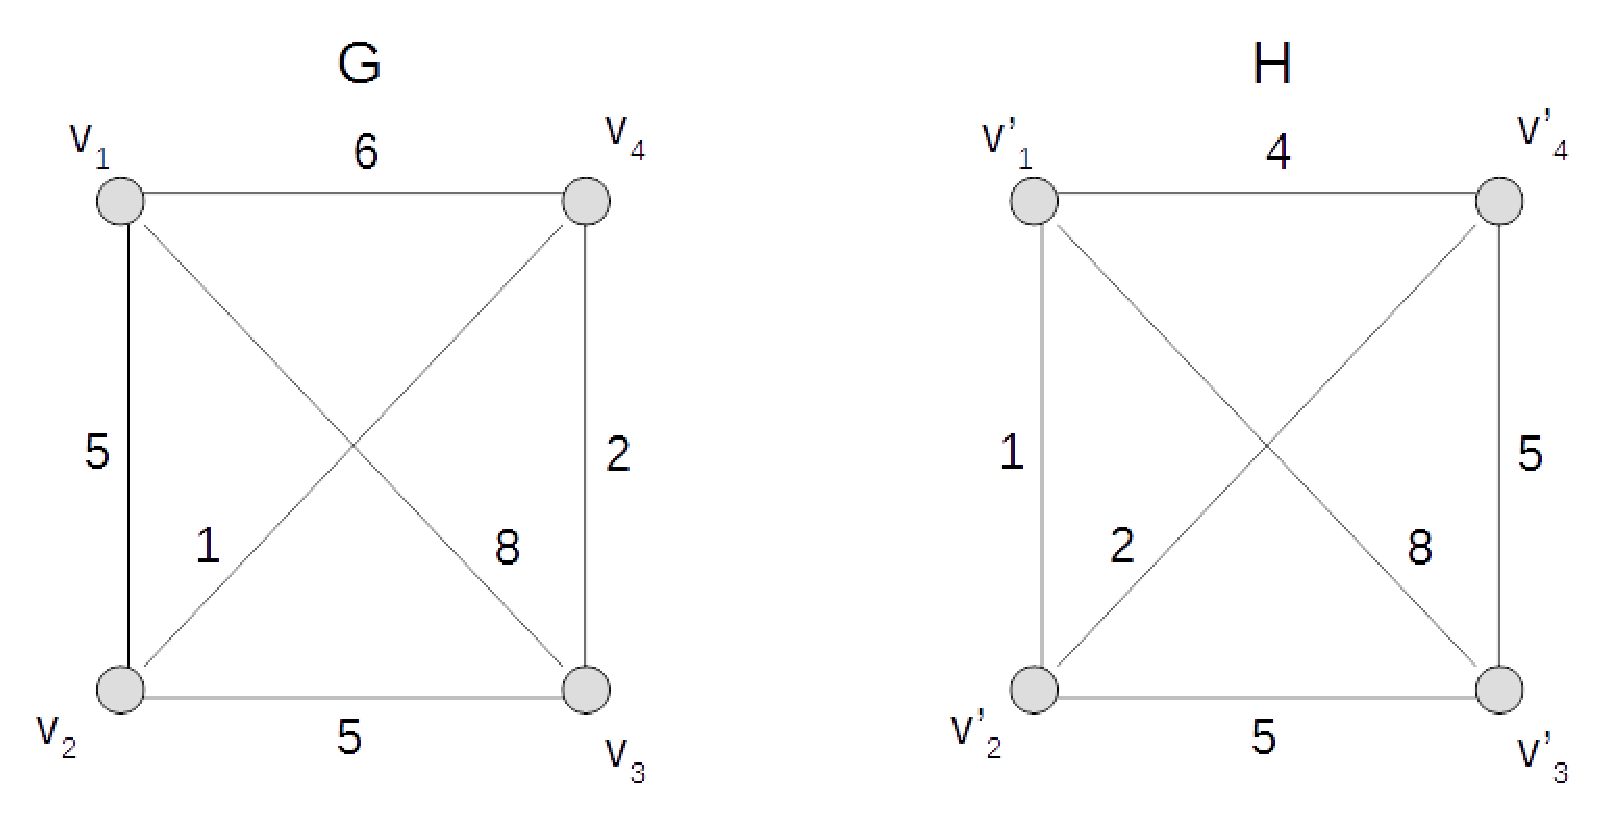
\includegraphics[width=12.5cm]{../images/gh.eps}
  \caption{グラフG、グラフH}
\end{figure}

図のグラフから隣接行列$A_G$、$A_H$は以下のようになる。
\begin{eqnarray}
  A_G=\begin{pmatrix}
    0.0 & 5.0 & 8.0 & 6.0 \\
    5.0 & 0.0 & 5.0 & 1.0 \\
    8.0 & 5.0 & 0.0 & 2.0 \\
    6.0 & 1.0 & 2.0 & 0.0
  \end{pmatrix} \notag \\
  A_H=\begin{pmatrix}
    0.0 & 1.0 & 8.0 & 4.0 \\
    1.0 & 0.0 & 5.0 & 2.0 \\
    8.0 & 5.0 & 0.0 & 5.0 \\
    4.0 & 2.0 & 5.0 & 0.0
  \end{pmatrix} \notag
\end{eqnarray}

得られた行列$A_G$、$A_H$をそれぞれ固有値分解する。この時、固有ベクトルを、対応する固有値の大きさ順に並べたモード行列を$U_G$、$U_H$とし、固有値を大きい順に対角上に並べた対角行列を$\Lambda_G$、$\Lambda_H$とすると以下の式のように表せる。
\begin{gather}
  \label{gaul}
  A_G=U_G\Lambda_GU_G^T \\
  \Lambda_G=diag(14.25,-0.28,-4.83,-9.14) \notag \\
  U_G=\begin{pmatrix}
    0.614 & 0.141 & -0.182 & -0.755 \\
    0.434 & -0.528 & 0.726 & 0.079 \\
    0.548 & -0.270 & -0.582 & 0.536 \\
    0.366 & 0.793 & 0.371 & 0.369
  \end{pmatrix} \notag \\
    \label{haul}
    A_H=U_H\Lambda_HU_H^T \\
    \Lambda_H=diag(13.26,-0.77,-3.43,-9.05) \notag \\
    U_H=\begin{pmatrix}
      0.538 & -0.436 & -0.425 & -0.583 \\
      0.344 & 0.880 & -0.018 & -0.327 \\
      0.624 & 0.026 & -0.250 & 0.740 \\
      0.450 & 0.187 & 0.870 & 0.079
    \end{pmatrix} \notag
\end{gather}
$U_G$、$U_H$のすべての要素の絶対値を取ると、行に各ノード、列に各固有値ベクトルが対応させることができる。
\begin{gather}
  \overline{U}_G=\begin{pmatrix}
    0.614 & 0.141 & 0.182 & 0.755 \\
    0.434 & 0.528 & 0.726 & 0.079 \\
    0.548 & 0.270 & 0.582 & 0.536 \\
    0.366 & 0.793 & 0.371 & 0.369
  \end{pmatrix} \notag \\
  \overline{U}_H=\begin{pmatrix}
    0.538 & 0.436 & 0.425 & 0.583 \\
    0.344 & 0.880 & 0.018 & 0.327 \\
    0.624 & 0.026 & 0.250 & 0.740 \\
    0.450 & 0.187 & 0.870 & 0.079
  \end{pmatrix} \notag
\end{gather}
行に各ノードというのはつまり、ノード数4の重み付き無向グラフを、隣接行列の固有値分解により4次元空間上で重みを距離に反映した四つの頂点に変換したことになる。

$A_G$と$A_H$が同型であると仮定すると、式(\ref{jp_p2})の左辺が0になる。よって、
\begin{equation}
  \label{pageah}
  PA_GP^T=A_H
\end{equation}
を満たす$P$が存在する。式(\ref{pageah})、(\ref{gaul})、(\ref{haul})より、
\begin{equation}
  PU_G\Lambda_GU_G^TP^T=U_H\Lambda_hU_H^T \notag
\end{equation}
再度、$A_G$、$A_H$が同型であるという仮定から
\begin{equation}
  PU_G=U_HS \notag
\end{equation}
を満たす行列$S$が存在し、
\begin{equation}
  P=U_HSU_G^T \notag
\end{equation}
と表せる。

求めたい$P$は順列行列であるから、$\hat{P}$を導入し、
\begin{eqnarray}
  \hat{P}=\bordermatrix{  & & \pi(i) \cr
                    & & \vdots \cr
                  i & \cdots & 1 \cr
                  } \notag
\end{eqnarray}
対角行列を$\hat{S}$とし、$U_H=[h_{ij}]$、$U_G=[g_{ij}]$、$\hat{S}=diag(s_i)$であることを用いて
\begin{equation}
  tr(\hat{P}^TU_H\hat{S}U_G^T)=\textstyle\sum\limits_{i=1}^{n}\textstyle\sum\limits_{j=1}^{n}s_jh_{ij}g_{\pi(i)j} \notag
\end{equation}
ここで、
\begin{equation}
  \begin{split}
  \sum_{j=1}^{n}s_jh_{ij}g_{\pi(i)j}&\le|\textstyle\sum\limits_{j=1}^{n}s_jh_{ij}g_{\pi(i)j} \notag \\
                                    &\le\textstyle\sum\limits_{j=1}^{n}|s_jh_{ij}g_{\pi(i)j} \notag \\
                                    &=\textstyle\sum\limits_{j=1}^{n}|h_{ij}||g_{\pi(i)j} \notag
  \end{split}
\end{equation}
よって、
\begin{equation}
  \begin{split}
    tr(\hat{P}^TU_H\hat{s}U_G^T)&\le\textstyle\sum\limits_{i=1}^{n}\textstyle\sum\limits_{j=1}^{n}|h_{ij}||g_{\pi(i)j}| \notag \\
          &=tr(\hat{P}\overline{U}_H\overline{U}_G^T) \notag
  \end{split}
\end{equation}

モード行列$U_G$、$U_H$は長さ1の固有ベクトルでできた行列であり、各要素の絶対値を取った$\overline{U}_G$、$\overline{U}_H$の行ベクトルも長さは1であるから、$\overline{U}_G\overline{U}_H=[x_{ij}]$とした時、$0\le x_{ij}\le1$を満たす。

以上より、任意の順列行列$P$は、
\begin{equation}
  tr(P^T\overline{U}_H\overline{U}_G^T)\le n \notag
\end{equation}
を満たし、$P$が最適マッチングを導く時、$n$が最大値となるので、$\overline{U}_H\overline{U}_G^T$に、ハンガリアン法を用いることで、最適な割り当てを求めている。

参考までに、ハンガリアン法を用いて求められた$P$は、
\begin{equation}
  P=\begin{pmatrix}
    0 & 0 & 1 & 0 \\
    0 & 0 & 0 & 1 \\
    1 & 0 & 0 & 0 \\
    0 & 1 & 0 & 0
  \end{pmatrix} \notag
\end{equation}

\subsection{ハンガリアン法}
\textbf{ハンガリアン法}(Hungarian method)とは、割当問題の解法として頻繁に用いられるものの一つであり、n次の正方行列が与えられた時、それぞれの行、列に重複が無いように値を選び出し、最小となる組合せを見つけるといった問題を解くことができる。たとえば、「n個の仕事をn人の作業員にやらせる時のコストを考える。同じ仕事を複数人の作業員でこなすことは無く、また、同じ作業員が複数の仕事をこなすこともないことを条件とし、仕事jを作業員iがやる時のコストを$c_{ij}$としたコスト行列Cを入力として、コストが最小になる割り当てを見つける」

グラフのノードマッチングを解く際は、最大となる組合せを見つけることになるが、予め行列の全要素を-1倍してから最小となる組合せを見つけることにし、最大化問題を最小化問題に置き換えている。

ハンガリアン法は、以下の6ステップにより構成される。
\begin{enumerate}
  \item 各行の最小値を、その行の全要素から引く。
  \item 各列の最小値を、その列の全要素から引く。
  \item 行列内のすべての0を通るように必要最小限数の直線を引き、直線状の要素に印をつける。
  \item $直線の本数=n$であれば、値が0の要素が最適マッチングの位置であり、終了。
  \item $直線の本数<n$であれば、印のないすべての要素の最小値を、印がないすべての要素から引き、印が二つついている要素には同じ値を加算する。
  \item 4に戻る。
\end{enumerate}
作業員に割り当てる際、作業員毎のコストの差が重要であり、差が同じであれば最適な割当ては変わらない点に注目している。

\subsection{まとめ}
梅山氏の提案手法で想定されている入力は、ノード数が一致しており、構造がほぼ同型なグラフであり、それ以外の、ノード数が一致しなかったり、グラフの構造が大きく異なっているもの同士のノードマッチングの精度は保証されないことに注意する必要がある。


\chapter{実験と考察}
本章では、実験の流れについて説明していく。

\section{目的}
本研究の目的は、word2vecの出力ベクトルを利用して語の相似関係を抽出することであり、この実験では、一対の単語ペアを入力とし、入力単語それぞれの近傍n個ずつの単語で作った二つのグループに梅山氏の提案手法を用いることでグループ内の単語同士の対応関係を出力する。

\section{実験データ}
用いた実験データについて説明する。

コーパスとして用いたのは、2016年9月時点での日本語版Wikipedia最新記事\footnote{https://dumps.wikimedia.org/jawiki/20160901/jawiki-20160901-pages-articles.xml.bz2}であり、ここからテキストデータを抽出し、MeCabを用いて形態素毎に分かち書きした。

次に、word2vecを用いて分かち書きしたコーパスから形態素の意味表現ベクトルを学習した。ベクトル学習のハイパーパラメータは以下の通りである。
\begin{itemize}
  \item 適用手法:CBoW
  \item 学習するベクトルの次元数:200
  \item 文脈窓:8
  \item 負例サンプリング数:25
  \item 階層型ソフトマックス:利用しない
  \item 学習の反復回数:15
\end{itemize}
文脈窓は、学習する際に使用する、対象語の前後の文脈語数で、今回文脈語は全部で16個使っている。

\section{梅山氏の手法の有効性確認}
まず初めに、word2vecの出力ベクトルデータを元に、単語同士の相似関係を梅山氏のグラフノードマッチング手法を利用して抽出できるかどうかを確認した。

表(\ref{test_pre})にある、集合X、集合Yの二つの単語群を作成した。これらは、男という括りにできる単語集合(X)と、女という括りにできる単語集合(Y)であり、それぞれ対になる単語が含まれるように作成した(例:父-母、雄-雌)。
\begin{table}[h]
  \begin{minipage}[t]{.45\textwidth}
    \caption[テストデータ]{手法の妥当性確認のためのテストデータ}
    \label{test_pre}
    \begin{center}
      \begin{tabular}{|c||c|} \hline
        集合X & 集合Y \\ \hline \hline
        叔父 & 妹 \\
        王 & 祖母 \\
        老人 & 王女 \\
        父 & 雌 \\
        兄 & 老婆 \\
        祖父 & 花子 \\
        弟 & 姉 \\
        息子 & 叔母 \\
        雄 & 娘 \\
        太郎 & 母 \\ \hline
      \end{tabular}
    \end{center}
  \end{minipage}
  \hfill
  \begin{minipage}[t]{.45\textwidth}
    \caption[テストデータのノードマッチング解析結果]{テストデータのノードマッチング解析結果}
    \label{test_bfr}
    \begin{center}
      \begin{tabular}{|c||c|} \hline
        集合X & 集合Y \\ \hline \hline
        叔父 & 叔母 \\
        王 & 王女 \\
        老人 & 老婆 \\
        父 & 母 \\
        兄 & 姉 \\
        祖父 & 祖母 \\
        弟 & 妹 \\
        息子 & 娘 \\
        雄 & 雌 \\
        太郎 & 花子 \\ \hline
      \end{tabular}
    \end{center}
  \end{minipage}
\end{table}

これらの集合を元に、word2vecが出力したベクトルをからなる行列$U_X$、$U_Y$を作成した。

\begin{equation}
  U_X=\begin{pmatrix}
    x_1 \\
    \vdots \\
    x_n
  \end{pmatrix} \notag \\
  \\
  U_Y=\begin{pmatrix}
    y_1 \\
    \vdots \\
    y_n
  \end{pmatrix} \notag \\
\end{equation}
$U_X$、$U_Y$はそれぞれ、第\ref{s_ts}節で述べた$U_G$、$U_H$に対応する。

集合Xの単語と、集合Yの単語は、それぞれのグループにおいて、二点間の距離が重みとして乗ったグラフとみて、$U_G$、$U_H$の代わりに$U_X$、$U_Y$を用いて、梅山氏の提案手法を適用した。この際、word2vecによる出力ベクトル空間において、単語ベクトルの長さが持つ情報が不明瞭であるため、余弦類似度をコスト行列作成に用いた。

グループX、Yに関して、梅山氏の提案手法によるノードマッチングを適用した結果が表(\ref{test_bfr})の通りであるから、ある括りで作られた単語グループ同士では、ほぼ同型のグラフ構造が得られ、梅山氏のノードマッチングの適用で対応する単語同士を発見できることと、word2vecの出力ベクトルは単語の相似関係を保持できていることが予想できる。

word2vecの学習がうまくできていることの確認と、学習ベクトルに梅山氏が提案したノードマッチング問題の解法を適用することで相似関係が抽出できることの確認のために、2013年にT.Mikolovらによって発表された論文に掲載されている下記のグラフ(\ref{ccv_pca_m})で見られる関係の抽出確認を行った。

\begin{figure}[!h]
  \centering
    \label{ccv_pca_m}
  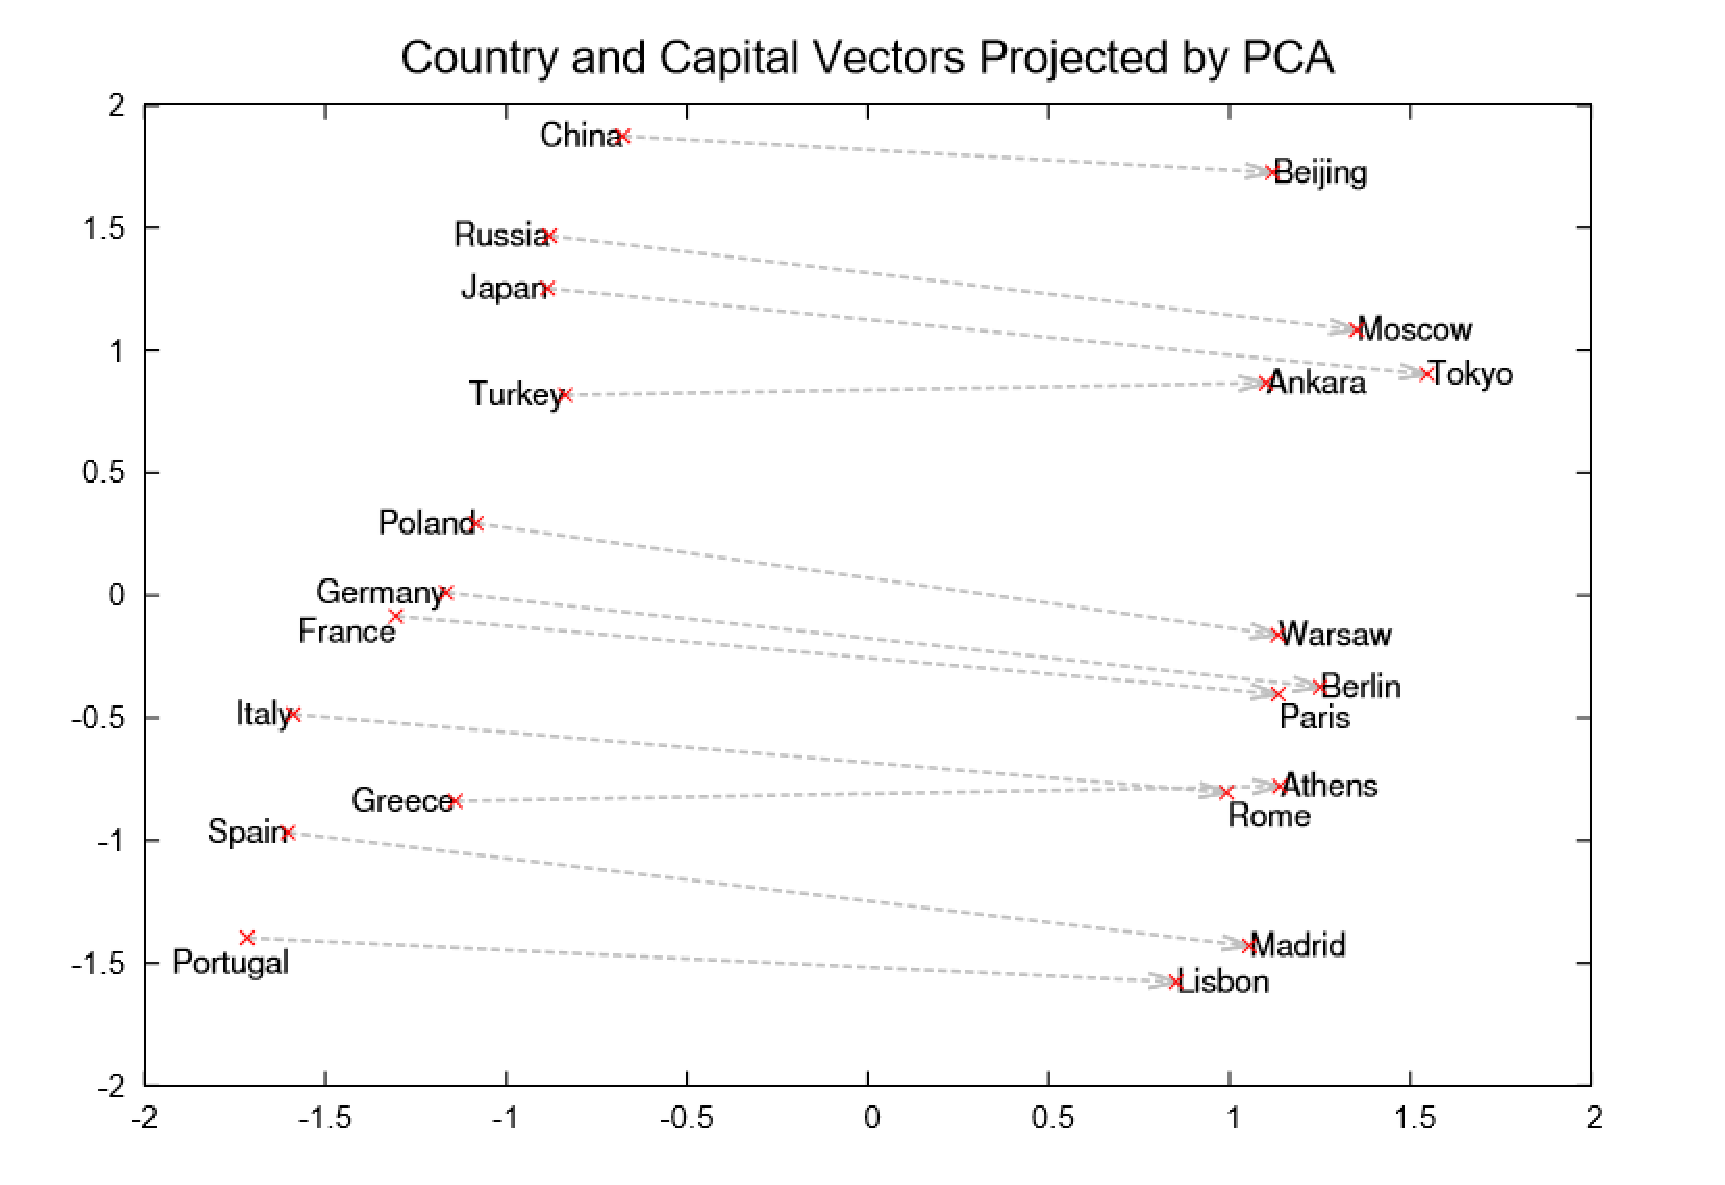
\includegraphics[width=12.5cm]{../images/CCVbyPCAfromM.eps}
  \caption[Country and Capital Vectors Projected by PCA(\cite{drwpc})]{連続Skip-gramモデルで学習した1000次元の単語ベクトルを、主成分分析により2次元に縮約し、いくつかの国名と首都名をプロットしたもの。首都名などの関係情報を与えること無しに、モデルが自動的に単語の概念を暗黙的に学習したことが見て取れる。\cite{drwpc}}
\end{figure}
このグラフにある例を用いて、先ほどと同様に単語集合を作りノードマッチングを行った結果が以下の表(\ref{ccv_c})である
\begin{table}[!h]
  \caption[国名と都市名のマッチング結果]{国名と都市名のマッチング結果}
  \label{ccv_c}
  \begin{center}
    \begin{tabular}{|c||c|} \hline
      集合X & 集合Y \\ \hline \hline
      中国 & 北京 \\
      ポーランド & ワルシャワ \\
      ギリシャ & アテネ \\
      ポルトガル & リスボン \\
      ドイツ & ベルリン \\
      スペイン & マドリード \\
      フランス & パリ \\
      ロシア & モスクワ \\
      トルコ & アンカラ \\
      日本 & 東京 \\
      イタリア & ローマ \\ \hline
    \end{tabular}
  \end{center}
\end{table}
これにより、グラフ(\ref{ccv_pca_m})で確認のできる対応関係と同等のものが抽出できていることがわかった。

グラフ(\ref{ccv_pca_m})\cite{drwpc}において、分散ベクトルの学習モデルは連続Skip-gramモデルで1000次元のベクトルを学習していたのに対し、本実験では学習モデルに連続Bag-of-Wordsモデルを用いて200次元のベクトルを学習していた。ハイパーパラメーターやモデルに差があったが、今回の検証実験により、低次元ベクトルにおいても単語の関係性が反映されていると期待できるので、このまま検証を続けていく。

\section{実験1:着目形態素の近傍形態素でノードマッチング}
次に、入力された単語対それぞれの近傍単語から取得した単語で作成したグループ同士にノードマッチングを適用することで、単語同士の掃除関係が抽出できるかを実験した。

入力した単語対の近傍10個を取得したものが、表()で、この表に対しノードマッチングを適用した結果が、表()である。\\
ここで、近傍の取り方については、着目単語との余弦類似度が高いものを類似度の高さ順に取ってきている。

\begin{table}[!h]
  \begin{minipage}[t]{.45\textwidth}
    \caption[(王,女王)の近傍10単語]{(王,女王)の近傍10単語}
    \label{}
    \begin{center}
      \begin{tabular}{|c||c|} \hline
        集合X & 集合Y \\ \hline \hline
        は王 & 王女 \\
        皇帝 & 王妃 \\
        に王 & 国王 \\
        国王 & エリザベス女王 \\
        君主 & ヴィクトリア \\
        大王 & 王 \\
        王妃 & 王子 \\
        伯 & エリザベス1世 \\
        聖王 & エリザベス2世 \\
        女王 & 王配 \\ \hline
      \end{tabular}
    \end{center}
  \end{minipage}
  \hfill
  \begin{minipage}[t]{.45\textwidth}
    \caption[(王,女王)の近傍10単語でグラフノードマッチング]{(王,女王)の近傍10単語でグラフノードマッチング}
    \label{}
    \begin{center}
      \begin{tabular}{|c||c|} \hline
        集合X & 集合Y \\ \hline \hline
        は王 & 王 \\
        皇帝 & 国王 \\
        女王 & ヴィクトリア \\
        \textbf{国王} & \textbf{エリザベス女王} \\
        に王 & 王妃 \\
        王妃 & 王配 \\
        君主 & 王子 \\
        \textbf{大王} & \textbf{王女} \\
        伯 & エリザベス1世 \\
        \textbf{聖王}\footnote{徳が深い王} & \textbf{エリザベス2世} \\ \hline
      \end{tabular}
    \end{center}
  \end{minipage}
\end{table}

結果を見るに、そもそも形態素解析がうまくできていない部分があったことがわかる。加えて、(王,女王)の関係にあるような対応関係を構築することが、人手でも難しい集合になってしまっていることがわかる。

他の例でもいくつか試してみた。
\begin{table}[!h]
  \begin{minipage}[t]{.45\textwidth}
    \caption[(日本,アメリカ)の近傍10単語]{(日本,アメリカ)の近傍10単語}
    \label{}
    \begin{center}
      \begin{tabular}{|c||c|} \hline
        集合X & 集合Y \\ \hline \hline
        韓国 & 米国 \\
        日本国内 & イギリス \\
        台湾 & 英国 \\
        中国 & カナダ \\
        欧米 & アメリカ合衆国 \\
        海外 & ヨーロッパ \\
        日本の文化 & オーストラリア \\
        日本国外 & フランス \\
        アジア & ドイツ \\
        わが国 & キューバ \\ \hline
      \end{tabular}
    \end{center}
  \end{minipage}
  \hfill
  \begin{minipage}[t]{.45\textwidth}
    \caption[(日本,アメリカ)の近傍10単語でグラフノードマッチング]{(日本,アメリカ)の近傍10単語でグラフノードマッチング}
    \label{}
    \begin{center}
      \begin{tabular}{|c||c|} \hline
        集合X & 集合Y \\ \hline \hline
        韓国 & オーストラリア \\
        欧米 & ヨーロッパ \\
        日本国内 & 米国 \\
        海外 & 英国 \\
        アジア & イギリス \\
        台湾 & キューバ \\
        中国 & ドイツ \\
        日本国外 & カナダ \\
        わが国 & フランス \\
        日本の文化 & アメリカ合衆国 \\ \hline
      \end{tabular}
    \end{center}
  \end{minipage}
\end{table}

\begin{table}[h]
  \begin{minipage}[t]{.45\textwidth}
    \caption[(東京,東京タワー)の近傍10単語]{(東京,東京タワー)の近傍10単語}
    \label{}
    \begin{center}
      \begin{tabular}{|c||c|} \hline
        集合X & 集合Y \\ \hline \hline
        大阪 & 東京スカイツリー \\
        名古屋 & 名古屋テレビ塔 \\
        関西 & スカイツリー \\
        札幌 & 電波塔 \\
        横浜 & 屋上 \\
        京都 & オカンとボクと、時々、オトン \\
        神戸 & ランドマークタワー \\
        静岡 & 六本木ヒルズ \\
        新潟 & タワー \\
        神奈川 & お台場 \\ \hline
      \end{tabular}
    \end{center}
  \end{minipage}
  \hfill
  \begin{minipage}[t]{.45\textwidth}
    \caption[(東京,東京タワー)の近傍10単語のグラフマッチング]{(東京,東京タワー)の近傍10単語のグラフマッチング}
    \label{}
    \begin{center}
      \begin{tabular}{|c||c|} \hline
        集合X & 集合Y \\ \hline \hline
        大阪 & お台場 \\
        札幌 & 六本木ヒルズ \\
        \textbf{名古屋} & \textbf{名古屋テレビ塔} \\
        \textbf{横浜} & \textbf{ランドマークタワー} \\
        新宿 & タワー \\
        関西 & 東京スカイツリー \\
        神奈川 & オカンとボクと、時々、オトン \\
        神戸 & スカイツリー \\
        静岡 & 電波塔 \\
        京都 & 屋上 \\ \hline
      \end{tabular}
    \end{center}
  \end{minipage}
\end{table}

\begin{table}[h]
  \begin{minipage}[t]{.45\textwidth}
    \caption[(北海道,札幌)の近傍10単語]{(北海道,札幌)の近傍10単語}
    \label{}
    \begin{center}
      \begin{tabular}{|c||c|} \hline
        集合X & 集合Y \\ \hline \hline
        道内 & 函館 \\
        札幌 & 小樽 \\
        十勝 & 旭川 \\
        釧路 & 帯広 \\
        東北地方 & 釧路 \\
        十勝支庁 & 札幌市 \\
        道東 & 北海道 \\
        道南 & 仙台 \\
        札幌市 & 新潟 \\
        道北 & 岩見沢 \\ \hline
      \end{tabular}
    \end{center}
  \end{minipage}
  \hfill
  \begin{minipage}[t]{.45\textwidth}
    \caption[(北海道,札幌)の近傍10単語のグラフマッチング]{(北海道,札幌)の近傍10単語のグラフマッチング}
    \label{}
    \begin{center}
      \begin{tabular}{|c||c|} \hline
        集合X & 集合Y \\ \hline \hline
        道内 & 北海道 \\
        釧路 & 釧路 \\
        札幌 & 函館 \\
        \textbf{十勝} & \textbf{帯広} \\
        札幌市 & 岩見沢 \\
        道東 & 旭川 \\
        十勝支庁 & 札幌市 \\
        \textbf{東北地方} & \textbf{仙台} \\
        道南 & 小樽 \\
        道北 & 新潟 \\ \hline
      \end{tabular}
    \end{center}
  \end{minipage}
\end{table}

いくつかのケースを試してみたところ、一組の単語対の近傍単語同士で作ったマッチング10組のうち、与えた単語対の関係と等しいものは平均すると2組程度の取得にとどまった。

正答率の低さの原因として考えられることは、そもそも、与えた単語対の関係を作れる単語が各グループに揃わないことが原因として考えられた。そこから、取得する近傍単語の数を増やし、単語対を作る際のバリエーションを増やせるようにして、再度実験を行った。

\begin{table}[h]
  \begin{minipage}[t]{.45\textwidth}
    \caption[(北海道,札幌)の近傍20単語のグラフマッチング]{(北海道,札幌)の近傍20単語のグラフマッチング}
    \label{}
    \begin{center}
      \begin{tabular}{|c||c|} \hline
        集合X & 集合Y \\ \hline \hline
        道内 & 北海道 \\
        釧路 & 釧路 \\
        札幌市 & 札幌市 \\
        札幌 & 函館 \\
        \textbf{十勝} & \textbf{帯広} \\
        \textbf{青森県} & \textbf{青森} \\
        根室 & 室蘭 \\
        \textbf{道東} & \textbf{北見} \\
        \textbf{九州} & \textbf{福岡} \\
        十勝支庁 & 旭川市 \\ \hline
        釧路市 & 岩見沢 \\
        \textbf{東北地方} & \textbf{仙台} \\
        胆振 & 江別 \\
        函館 & 名古屋 \\
        道南 & 旭川 \\
        空知 & 丘珠 \\
        道北 & 苫小牧 \\
        道外 & 小樽 \\
        留萌 & 新潟 \\
        沖縄県 & 東京 \\ \hline
      \end{tabular}
    \end{center}
  \end{minipage}
  \hfill
  \begin{minipage}[t]{.45\textwidth}
    \caption[(東京,東京タワー)の近傍20単語のグラフマッチング]{(東京,東京タワー)の近傍20単語のグラフマッチング}
    \label{ttt}
    \begin{center}
      \begin{tabular}{|c||c|} \hline
        集合X & 集合Y \\ \hline \hline
        \textbf{大阪} & \textbf{通天閣} \\
        新宿 & サンシャイン60 \\
        名古屋 & お台場 \\
        日比谷 & スカイツリー \\
        関西 & 日本電波塔 \\
        札幌 & 六本木ヒルズ \\
        \textbf{横浜} & \textbf{ランドマークタワー} \\
        赤坂 & 大阪タワー \\
        静岡 & FCGビル \\
        神奈川 & ビル街 \\ \hline
        福岡 & 東京スカイツリー \\
        麹町 & 名古屋テレビ塔 \\
        神戸 & 屋上 \\
        都内 & オカンとボクと、時々、オトン \\
        埼玉 & 電波塔 \\
        京都 & 銀座和光 \\
        愛知 & テレビ塔 \\
        青山 & タワー \\
        渋谷 & 展望台 \\
        金沢 & 鉄塔 \\ \hline
      \end{tabular}
    \end{center}
  \end{minipage}
\end{table}

取得する近傍単語を増やしてノードマッチングを行った結果を確認したが、精度の上昇は見られなかった。原因として、与える単語対が近い位置関係にあり、それぞれの近傍として取得する単語が重複したことにより、同一単語でのマッチングが増え、事実上単語対が消失してしまった。

それ以外のケースにおいては、近傍単語の特徴にばらつきがあることがあげられる。

上記の表(\ref{ttt})においては、(東京,東京タワー)から、(地名,塔などの名所)といった関係の取得を想定していたが、それぞれから取得した近傍単語を見るに、"東京"の近傍には地名が多く出現し、想定通りであったが、"東京タワー"の近傍は"名所"、"塔"、"高所"、"題材とした映画"など、大きくぶれてしまった。これは、元にした"東京タワー"という単語が、名所、シンボル、建造物、イメージなど多岐にわたる意味を含有していたからだと推測される。

また、近傍の取得数が10個の時から出現していた映画タイトルについては、コーパス中の出現回数が31回と、他の単語の出現率の10分の1以下\footnote{鉄塔:570回、東京タワー:610回出現}であり、学習が十分になされなかったためにノイズ的に現れてしまったと認識できる。

\section{実験2:近傍単語をクラスタリングし、クラスター同士のマッチングを見る}
先の実験において、入力した一組の単語対それぞれから得た近傍単語同士のマッチングにより、入力単語対と相似な関係の取得は、近傍単語として取得できる単語の特徴に偏りがあることからよい結果が得られなった。

近傍単語の特徴に偏りがあることを考慮して、取得単語数を増やしてみた場合においても、近傍として設定した領域の重なりや、偏りが解消されないといった問題があった。そこで、偏りを解消するために近傍として取得する単語数を増やし、それぞれで同数のクラスターを作成し、クラスター同士のマッチングを考えた。



\begin{table}[h]
  \begin{minipage}[t]{.45\textwidth}
    \caption["日本"の近傍1000単語を20個のクラスターに分割した様子]{"日本"の近傍1000単語を20個のクラスターに分割した様子}
    \label{}
    \begin{center}
      \begin{tabular}{|c||c|} \hline
        クラスター No. & クラスターの特徴 \\ \hline \hline
        0 & ひらがな(名前) \\
        1 & アジアの国々とその関連  \\
        2 & 文明史など歴史関連語  \\
        3 & 日本史用語類  \\
        4 & ひらがな(意味不明瞭)  \\
        5 & ひらがな(人名) \\
        6 & 人名、日本史用語 \\
        7 & 地理科目系用語 \\
        8 & 国内の地名 \\
        9 & 大学、人名など \\
        10 & 日本-世界に関わる歴史用語 \\ \hline
        11 & 地域、国名 \\
        12 & ひらがな(苗字) \\
        13 & 日系、関連語 \\
        14 & 食 \\
        15 & 地域名、沖縄関連語 \\
        16 & 職業名○○家など \\
        17 & 分野別学者などの肩書 \\
        18 & 団体名、経済用語 \\
        19 & ひらがな(名前) \\ \hline
      \end{tabular}
    \end{center}
  \end{minipage}
  \hfill
  \begin{minipage}[t]{.45\textwidth}
    \caption["アメリカ"の近傍1000単語を20個のクラスターに分割した様子]{"アメリカ"の近傍1000単語を20個のクラスターに分割した様子}
    \label{}
    \begin{center}
      \begin{tabular}{|c||c|} \hline
        クラスター No. & クラスターの特徴 \\ \hline \hline
        0 & 地域、職業名、歴史用語など雑多 \\
        1 & アメリカ関連 人・地名 \\
        2 & 地域名、地理用語 \\
        3 & 商業、政策関連 \\
        4 & アメリカ地域名、問題など \\
        5 & アメリカ系地名 \\
        6 & 地域名、政治 \\
        7 & アメリカ史、人名 \\
        8 & 地名、経済 \\
        9 & 史学系用語 \\
        10 & 州単位の事件など \\ \hline
        11 & 地名、アメリカ国家間問題 \\
        12 & アメリカ系政治用語 \\
        13 & 地名、世界史 \\
        14 & 人権史 \\
        15 & 経済 \\
        16 & 地名 \\
        17 & 政治的世界史用語 \\
        18 & アメリカ-他国間 \\
        19 & 戦争など争い事。 \\ \hline
      \end{tabular}
    \end{center}
  \end{minipage}
\end{table}

\begin{table}[h]
  \caption["日本"のクラスターと"アメリカ"のクラスターの対応関係]{"日本"のクラスターと"アメリカ"のクラスターの対応関係}
  \label{}
  \begin{center}
    \begin{tabular}{|c||c|} \hline
      クラスター No.(日本) & クラスター No.(アメリカ) \\ \hline \hline
      0 & 16 \\
      1 & 17 \\
      2 & 6 \\
      3 & 12 \\
      4 & 2 \\
      5 & 14 \\
      6 & 7 \\
      7 & 3 \\
      8 & 11 \\
      9 & 18 \\ \hline
      10 & 4 \\
      11 & 5 \\
      12 & 19 \\
      13 & 1 \\
      14 & 10 \\
      15 & 8 \\
      16 & 0 \\
      17 & 9 \\
      18 & 15 \\
      19 & 13 \\ \hline
    \end{tabular}
  \end{center}
\end{table}

\begin{table}[h]
  \begin{minipage}[t]{.45\textwidth}
    \caption[]{}
    \label{}
    \begin{center}
      \begin{tabular}{|c||c|} \hline
        集合X & 集合Y \\ \hline \hline
         &  \\
         &  \\
         &  \\
         &  \\
         &  \\
         &  \\
         &  \\
         &  \\
         &  \\
         &  \\ \hline
      \end{tabular}
    \end{center}
  \end{minipage}
  \hfill
  \begin{minipage}[t]{.45\textwidth}
    \caption[]{}
    \label{}
    \begin{center}
      \begin{tabular}{|c||c|} \hline
        集合X & 集合Y \\ \hline \hline
         &  \\
         &  \\
         &  \\
         &  \\
         &  \\
         &  \\
         &  \\
         &  \\
         &  \\
         &  \\ \hline
      \end{tabular}
    \end{center}
  \end{minipage}
\end{table}

この実験を始めるにあたって、まず、近傍単語の様子を確認した。

\begin{table}[h]
  \begin{minipage}[t]{.45\textwidth}
    \caption[(王,女王)]{(王,女王)の近傍単語}
    \label{kq_table}
    \begin{center}
      \begin{tabular}{|c|c|} \hline
        王 & 女王 \\ \hline
        は王 & 王女 \\
        皇帝 & 王妃 \\
        に王 & 国王 \\
        国王 & エリザベス女王 \\
        君主 & ヴィクトリア \\
        大王 & 王 \\
        王妃 & 王子 \\
        伯 & エリザベス1世 \\
        聖王 & エリザベス2世 \\
        女王 & 王配 \\ \hline
      \end{tabular}
    \end{center}
  \end{minipage}
  \hfill
  \begin{minipage}[t]{.45\textwidth}
    \caption[(日本,アメリカ)]{(日本,アメリカ)の近傍単語}
    \begin{center}
      \begin{tabular}{|c|c|} \hline
        日本 & アメリカ \\ \hline
        韓国 & 米国 \\
        日本国内 & イギリス \\
        台湾 & 英国 \\
        中国 & カナダ \\
        欧米 & アメリカ合衆国 \\
        海外 & ヨーロッパ \\
        日本の文化 & オーストラリア \\
        日本国外 & フランス \\
        アジア & ドイツ \\
        わが国 & キューバ \\ \hline
      \end{tabular}
    \end{center}
  \end{minipage}
\end{table}

\newpage

表(\ref{kq_table})に関して、下図にあるような、(男,女)の関係に相当する単語が出力されることを想定していたため、この時点では大きな誤算である。
\begin{figure}[h]
  \centering
  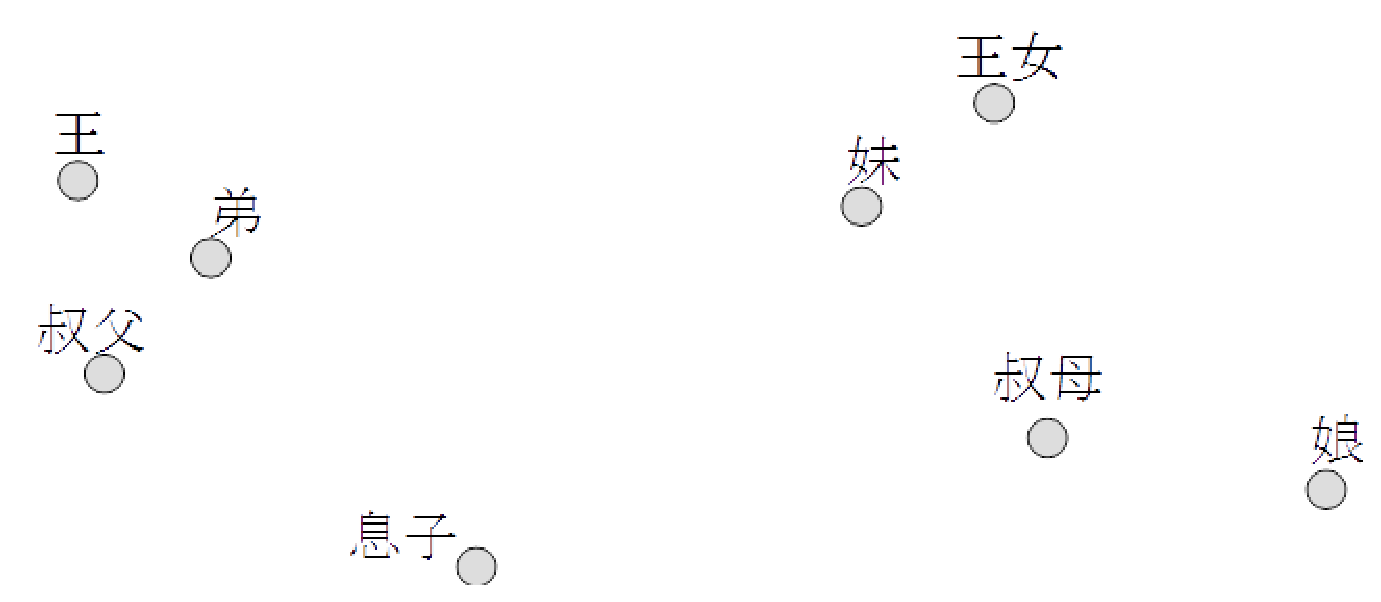
\includegraphics[width=8cm]{../images/kq_fv.eps}
  \caption{王-女王 近傍イメージ}
  \label{kq_fv}
\end{figure}

\begin{table}[h]
  \begin{minipage}[t]{.33\textwidth}
    \caption[(明るい,暗い)]{(明るい,暗い)の近傍単語}
    \begin{center}
      \begin{tabular}{|c|c|} \hline
        暗い & 明るい \\ \hline
        明るく & 暗く \\
        暗く & 明るく \\
        濃い & 薄暗い \\
        淡い & 眩しく \\
        眩しく & 青白い \\
        青白い & 濃い \\
        淡く & 薄暗く \\
        明るめ & 淡い \\
        鮮やか & ぼんやり \\ \hline
      \end{tabular}
    \end{center}
  \end{minipage}
  \begin{minipage}[t]{.66\textwidth}
    \caption[(光,影,闇)]{(光,影,闇)の近傍単語}
    \begin{center}
      \begin{tabular}{|c|c|c|} \hline
        太陽光 & 影の & 暗黒 \\ \hline
        反射 & 闇 & 妖魔 \\
        発光 & 暗闇 & 魔物 \\
        光線 & 暗部 & 邪悪 \\
        鏡 & 影 & 魔神 \\
        光源 & 暗い & 影 \\
        紫外線 & 隠れ & 悪魔 \\
        い光 & 暗黒 & 魔王 \\
        透かす & 其面 & 魔界 \\
        太陽 & 潜む & 魔 \\ \hline
      \end{tabular}
    \end{center}
  \end{minipage}
\end{table}
以上の結果を見るに、単純に近傍単語を同数取ってきたグループで作成するグラフは、与えた単語対が持つ関係を保持した同型のグラフには必ずしもなっていないことが予想される。


\chapter{結び}


\chapter*{謝辞}
本研究を進めるにあたって、特別な事情により普通よりも長い期間、丁寧にご指導いただきました原口先生に心から御礼申し上げます。
長い期間の在籍も、研究室内でサポートくださいました大久保先生、配属時の事情など御心配戴きました吉
岡先生にも、厚く御礼申し上げます。

研究を様々な面でサポートしていただきました先輩方、研究室の皆様にも大変お世話になりました。

未熟な私がここまでやってこれたのは、サポートしていただきました皆様のおかげであり、すべての方々に感謝を申し上げます。

\begin{flushright}
\end{flushright}


\cleardoublepage



\appendix


\bibliographystyle{jplain}
\bibliography{skb}

\end{document}
